\subsection{Test af programmet}
\label{sec:test}

Som en del af problemløsningen udføres der test på det udviklede program. Formålet med testafsnittet er, at undersøge om programmet lever op til de programkrav, som blev opstillet i slutningen af teoridiskussion, \ref{sec:teori}. Testene vil være med til at belyse eventuelle fejl og mangler i programmet.

Først testes det om programmet kan rendere et billede af en lampe og dens belysning. Dette gøres ved at sammenligne et billede taget med et fysisk kamera, med et billede renderet af programmet.

På figur \ref{fig:real} er der vist et billede taget med et mobilkamera (Samsung Galaxy S3), hvorimod billedet på figur \ref{fig:fake} er renderet af programmet på baggrund af en tilnærmet model af lampen, med nedenstående programparametre.
\begin{lstlisting}
./trace model.ply -V 0.785 -t 2700 -w 540 -h 960
\end{lstlisting}

\begin{figure}[H]
\centering
\begin{subfigure}{.5\textwidth}
  \centering
  \includegraphics[width=.6\linewidth]{real}
  \caption{Fotografi}
  \label{fig:real}
\end{subfigure}%
\begin{subfigure}{.5\textwidth}
  \centering
  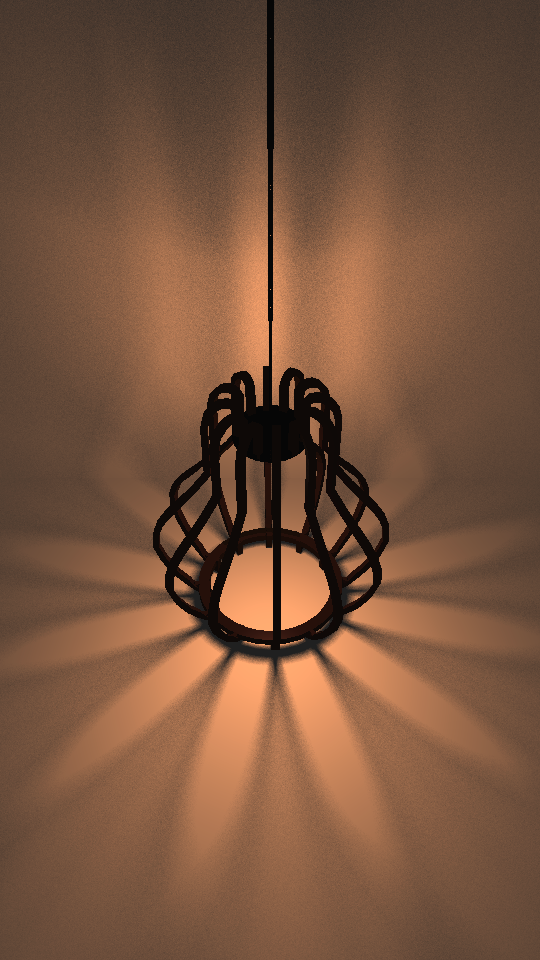
\includegraphics[width=.6\linewidth]{result_5305s}
  \caption{Renderet billede}
  \label{fig:fake}
\end{subfigure}
\caption{Viser billede taget med mobilkamera (a) og billede renderet af programmet (b). For de to billeder gælder at pærens farvetemperatur er angivet som 2700K.}
\label{fig:test_real_fake}
\end{figure}

For at teste de forskellige programparametre, som kan indtastes i programmet, er der herunder billeder af test med forskellige programparametre.

\subsubsection{Test af farvetemperatur}
\begin{figure}[H]
\centering
\begin{subfigure}{.5\textwidth}
  \centering
  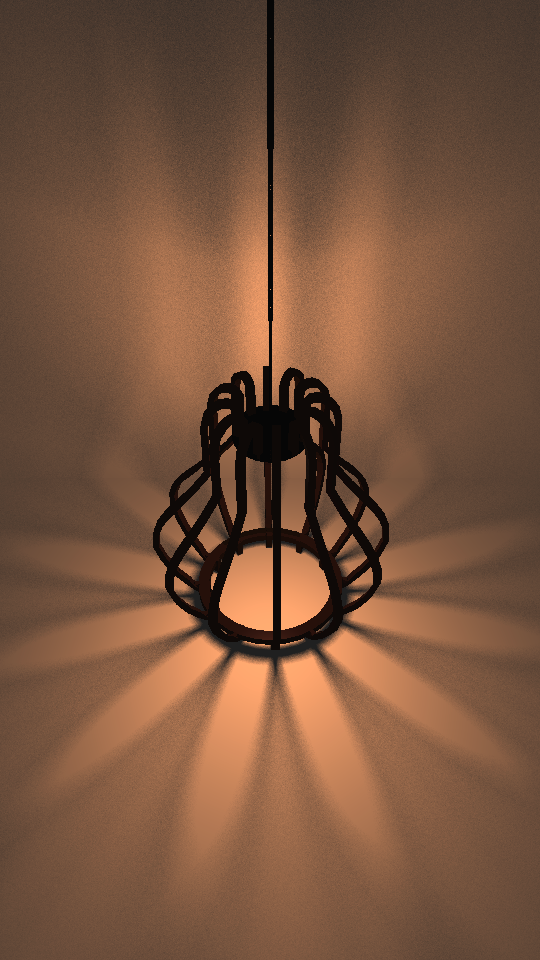
\includegraphics[width=.5\linewidth]{result_5305s}
  \caption{Farvetemperatur: 2700K}
  \label{fig:kelvin2700}
\end{subfigure}%
\begin{subfigure}{.5\textwidth}
  \centering
  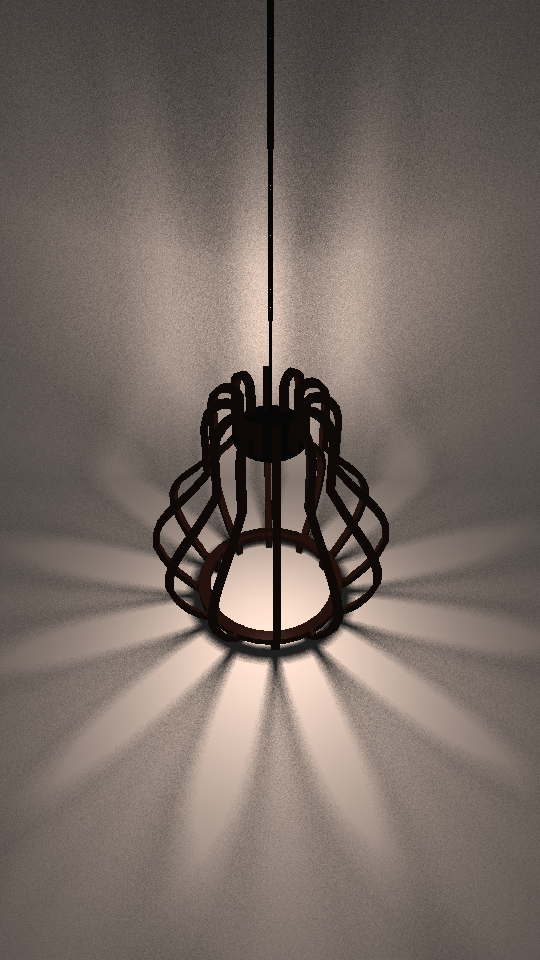
\includegraphics[width=.5\linewidth]{result_2734s_5000k_0H_0-785V}
  \caption{Farvetemperatur: 5000K}
  \label{fig:kelvin5000}
\end{subfigure}
\caption{Viser billede renderet af programmet med to forskellige farvetemperaturer.}
\label{fig:farvetemperatur}
\end{figure}

\subsubsection{Test af synsvinkler}
\begin{figure}[H]
\centering
\begin{subfigure}{.5\textwidth}
  \centering
  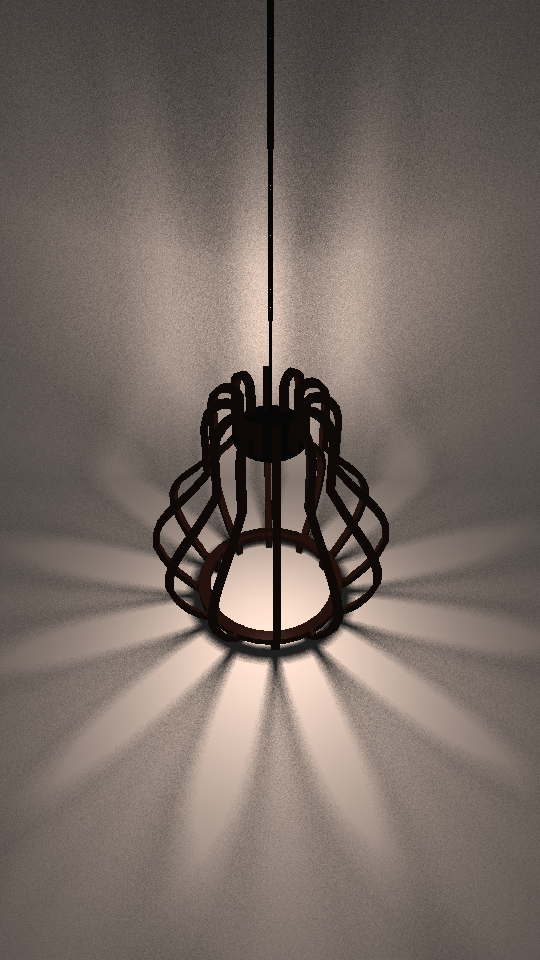
\includegraphics[width=.5\linewidth]{result_2734s_5000k_0H_0-785V}
  \caption{Horisontal vinkel: $0^o$ \\ Vertikal vinkel: $~45^o$}
  \label{fig:one}
\end{subfigure}%
\begin{subfigure}{.5\textwidth}
  \centering
  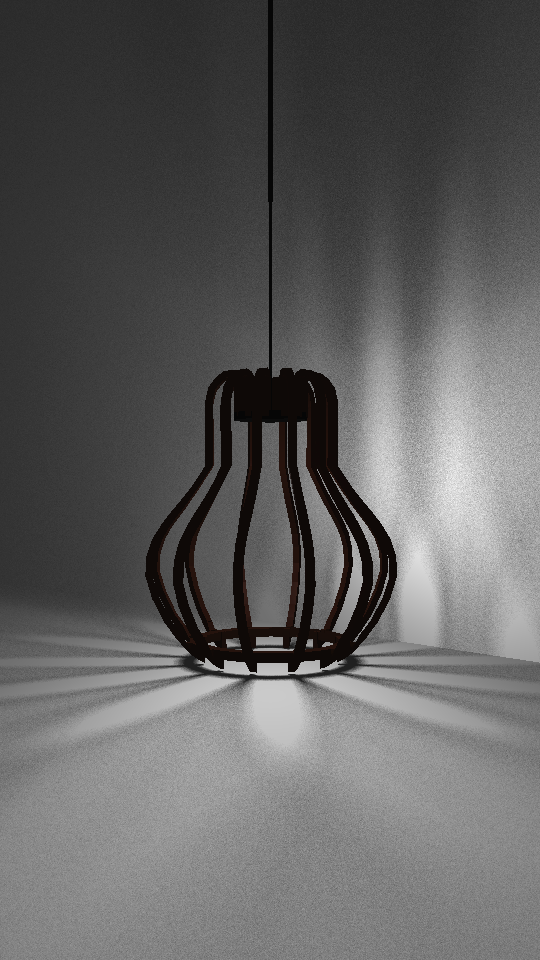
\includegraphics[width=.5\linewidth]{result_2758s_white_0-8H}
  \caption{Horisontal vinkel: $~45^o$ \\ Vertikal vinkel: $0^o$}
  \label{fig:two}
\end{subfigure}
\caption{Viser billeder renderet af programmet, med to forskellige vinkler.}
\label{fig:synsvinkel}
\end{figure}

\subsubsection{Test af optimering}
\begin{figure}[H]
\centering
\begin{subfigure}{.5\textwidth}
  \centering
  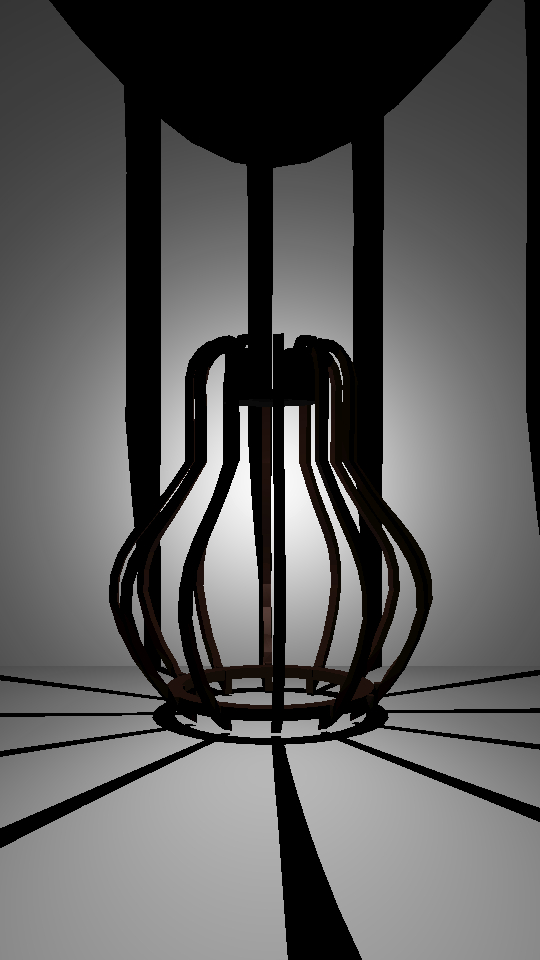
\includegraphics[width=.5\linewidth]{result658s}
  \caption{Før optimering: 658 sek.}
  \label{fig:slow}
\end{subfigure}%
\begin{subfigure}{.5\textwidth}
  \centering
  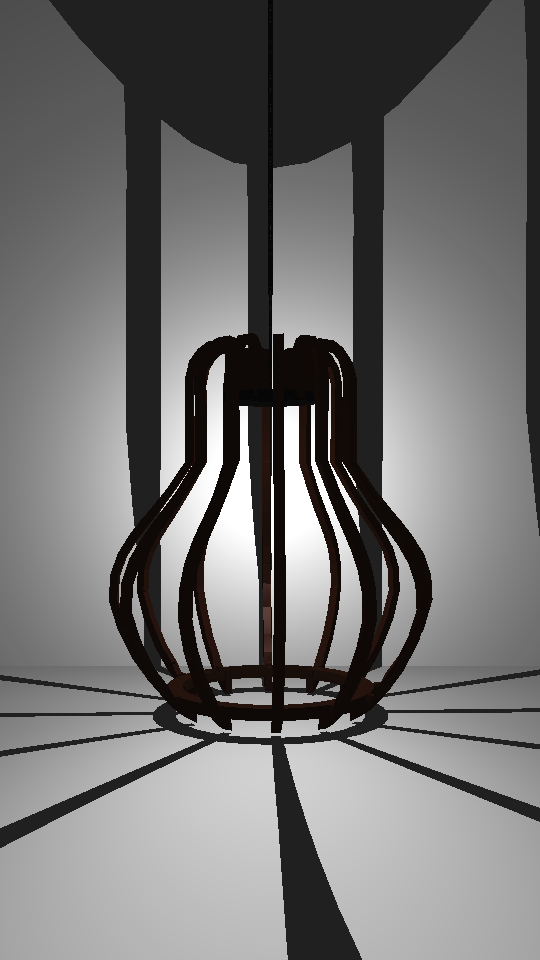
\includegraphics[width=.5\linewidth]{result53s}
  \caption{Efter optimering: 53 sek.}
  \label{fig:fast}
\end{subfigure}
\caption{Viser et billede angivet med renderingstider for programmet henholdsvis før og efter implementationen af KD-træer. Begge billeder er renderet uden bløde skygger.}
\label{fig:optimering}
\end{figure}


Med den gamle version af programmet opnås der en renderingstid på 658 sekunder, og med den nye version af programet opnås der en renderingstid på 53 sekunder. Der er altså efter implementationen af KD-træer, i dette tilfælde, opnået en speedup på $658 sek./53 sek. \approx 12$. Renderingen af de to billeder er foretaget på samme hardware, da renderingstiden bla.\ er afhængig af hvilken hardware programmet bliver kørt på. Hvis billederne renderes på anden hardware vil renderingstiden derfor ændres, men speedup skulle gerne være det samme. 


\subsection*{Opsummering}
Som vist på figur \ref{fig:fake} opfylder programmet krav 1-3 fra afsnit \ref{sec:krav_til_kode}, da den kan rendere og gemme et billede af en lampe og dens belysning på baggrund af indtastede input der indeholder 3D-fil, farvetemperatur, synsvinkel og opløsningen af billedet. Derudover er der, som vist, sket en optimering af programmets renderingstid efter implementeringen af KD-træer. 
Som det er vist på figur \ref{fig:test_real_fake} er der en afvigelse mellem billedet af den rigtige lampe og det renderede billede af en model af lampen. Denne afvigelse diskuteres i næste afsnit sammen med rapportens resterende resultater. 

%Der er nu blevet udført forskellige test af programmet, som senere diskuteres i afsnit \ref{sec:diskussion}.